%
% HSR LaTex Template
% Copyright 2012, Florian Bentele / modified 2015 - Martin Stypinski
%
% Complete LaTex template for thesis at HSR, customized
% for Prof. Dr. Peter Heinzmann
%
%
% This document is free software: you can redistribute
% it and/or modify it under the terms of the GNU
% General Public License as published by the Free
% Software Foundation, either version 3 of the License,
% or (at your option) any later version.
%
% This document is distributed in the hope that it will
% be useful, but WITHOUT ANY WARRANTY; without even the
% implied warranty of MERCHANTABILITY or FITNESS FOR A
% PARTICULAR PURPOSE. See the GNU General Public
% License for more details.
%
% You should have received a copy of the GNU General
% Public License along with this document. If not, see
% <http://www.gnu.org/licenses/>.
%

\newcommand{\kiru}{Kirusanth Poopalasingam}
\newcommand{\styp}{Martin Stypinski}
\newcommand{\aeme}{Marcel Amsler}

\documentclass[11pt]{hsrthesis}

\makeindex


\begin{document}
\newcommand{\thesistitle}{Project Helin}
\newcommand{\thesisauthora}{Marcel Amsler}
\newcommand{\thesisauthorb}{Kirusanth Poopalasingam}
\newcommand{\thesisauthorc}{Martin Stypinski}
\newcommand{\professor}{Prof. Dr. Markus Stolze}
\newcommand{\thesistype}{Bachelorarbeit}
\newcommand{\departement}{Abteilung Informatik}
\newcommand{\school}{Hochschule für Technik Rapperswil}
\newcommand{\term}{Frühlingssemester 2016}
\newcommand{\thedate}{29. Mai 2015}
\newcommand{\timeperiode}{16.02.2015 - 29.05.2015}
\newcommand{\workload}{360 Stunden, 12 ECTS pro Student}
\newcommand{\linktothesis}{https://github.com/Project-Helin/}

\maketitle


\newpage

\pagenumbering{roman}


% The main content
%%%%%%%%%%%%%%%%%%


\cleardoublepage
\phantomsection
\addcontentsline{toc}{chapter}{Eigenständigkeitserklärung}
\chapter*{Eigenständigkeitserklärung}

%\chapter{Eigenständigkeitserklärung}
Wir erklären hiermit,
\begin{itemize}
	\item{dass wir die vorliegende Arbeit selber und ohne fremde Hilfe durchgeführt haben, ausser
derjenigen, welche explizit in der Aufgabenstellung erwähnt sind oder mit dem Betreuer
schriftlich vereinbart wurden,}
	\item{dass wir sämtliche verwendeten Quellen erwähnt und gemäss gängigen wissenschaftlichen
Zitierregeln korrekt angegeben haben,}
	\item{dass wir keine durch Copyright geschätzten Materialien (z. B. Bilder) in dieser Arbeit in
unerlaubter Weise genutzt haben.}
\end{itemize}
\begin{verbatim}




\end{verbatim}
Rapperswil, den \today
\begin{verbatim}







\end{verbatim}
\centering
\includegraphics[width=1.0\paperwidth]{unterschriften/alle.jpg}
\begin{tabular*}{\textwidth}{p{0cm}>{\centering\arraybackslash}m{4.8cm}>{\centering\arraybackslash}m{4.8cm}>{\centering\arraybackslash}m{4.8cm}p{0cm}}
	& Marcel Amsler & Kirusanth Poopalasingam & Martin Stypinski & \\
\end{tabular*}

\newpage
\addcontentsline{toc}{chapter}{Danksagung}
\chapter*{Danksagung}
Zunächst möchten wir uns an dieser Stelle bei all denjenigen bedanken, die uns während der Anfertigung dieser Arbeit unterstützt und motiviert haben.
\begin{itemize}
	\item{}
\end{itemize}
\newpage
\addcontentsline{toc}{chapter}{Abstract}
\chapter*{Abstract}
YOLO Abstract 1
\newpage
\cleardoublepage
\phantomsection
\addcontentsline{toc}{chapter}{Management Summary}
\chapter*{Management Summary}
\section*{Ausgangslage}
Drohnen, die autonom fliegen und nicht mehr gesteuert werden müssen, gehört die Zukunft. Sie werden sicherer sein als heutige, von Menschen gesteuerte Drohnen und erlauben ein grösseres Einsatzgebiet. Firmen wie Amazon und die schweizerische Post planen bereits heute den Einsatz von Drohnen zur automatischen Auslieferung von Paketen. Doch vielen Anbietern bleibt diese Möglichkeit verwehrt, obwohl auf dem Markt eine Vielzahl von Komponenten zur Verfügung steht, um autonome Drohnen selbst zu bauen und zu betreiben. Die bestehenden Lösungen steuern aber immer nur eine Drohne gleichzeitig über Funk und bieten nur eine begrenzte Reichweite. Ausserdem existiert noch keine frei verfügbare Software, um automatisierte Dienstleistungen mit Drohnen anzubieten oder eine autonome Flotte zu verwalten.

\section*{Vorgehen / Technologien}
Um zu zeigen, was mit heutigen Technologien und Standardkomponenten bereits möglich ist, wurde ein Demonstrationssystem mit zwei selbst gebauten Drohnen entwickelt. \\

Ein Smartphone, welches auf der Drohne montiert ist, ermöglicht die Kommunikation mit der Plattform, aber auch eine Benutzerinteraktion über das Display. Bei einer eingehenden Bestellung von der Bestell-App wird automatisch eine Route zum Kunden berechnet und einer verfügbaren Drohne zugewiesen. Sobald diese beladen ist, fliegt sie autonom zum Kunden, liefert das Produkt aus und kehrt wieder zurück. Dabei bleibt die Drohne in den vordefinierten, sicheren Flugzonen und weicht somit statischen Hindernissen aus. Eine Fernsteuerung wird nicht mehr benötigt, das System ist komplett autonom. Die App dient als Schnittstelle zwischen der cloudbasierten Verwaltungssoftware und der Drohnensteuerung, welche bereits grundsätzliche Funktionen wie GPS, automatische Stabilisierung und sogar einen programmierbaren Autopiloten bietet.

\section*{Ergebnisse}
Das System zeigt erst einen Bruchteil der Möglichkeiten, die in Zukunft von autonomen Drohnen übernommen werden können. Beispielsweise können Videoaufnahmen, Infrastrukturüberwachung oder Katastrophenhilfe als Angebote integriert werden. \\

Wir sind überzeugt davon, dass die entwickelte Plattform als Denkanstoss für diese Branche und die Politik dienen kann, um die Technologien und Gesetzeslagen soweit zu verbessern, dass Dienstleistungen von Drohnen bald überall zur Verfügung stehen werden.

\newpage
\addcontentsline{toc}{chapter}{Aufgabenstellung}
\chapter*{Aufgabenstellung}
\label{cha:aufgabenstellung}

\section*{Betreuer \& Auftraggeber}
\begin{itemize}
	\item{\textbf{Betreuer:} Prof Dr. Markus Stolze, Dozent für Informatik HSR}
	\item{\textbf{Co-Referent:} Prof Beat Stettler, Dozent für Informatik HSR}
	\item{\textbf{Experte:} TBD}
	\item{\textbf{Anwendungspartner:} Abteilung Informatik HSR}		
\end{itemize}

\section*{Ausgangslage}
Multicopter haben in den letzten Jahren grosse technologische Fortschritte erlebt. Sie sind leichter, einfacher zu bedienen, leistungsfähiger und preiswerter geworden, so dass sie auch für kleine Geschäfte und Privatpersonen erschwinglich geworden sind. 
Ein möglicher Anwendungsbereich von Multicoptern ist die schnelle Auslieferung von Produkten. So ist es im Prinzip schon heute möglich mit einem Multicopter einen Defibrillator punktgenau zu einer bedürftigen Person an einem Open-Air-Konzert zu bringen. Allerdings erlaubt die aktuelle Gesetzgebung keine automatisch gesteuerten Flüge von Multicoptern. Zudem ist auch manuell gesteuerte Flüge „auf Sicht“ in der Nähe von grösseren Menschenansammlungen nicht erlaubt. Da die Gesetzliche Lage aktuell im Fluss ist, kann es sein dass diese Limitationen schon bald nicht mehr gelten und es somit interessant wäre eine Software-Platform zu erstellen mit der automatisch gesteuerte Zustellung von Produkten mit Multicoptern abgewickelt werden können.  

\section*{Ziele der Arbeit}
In dieser Arbeit sollen Komponenten eine erweiterbare open-source Software-Plattform mit den folgenden vier Komponenten erstellt werden 
\begin{enumerate}
	\item{Ein Prototyp einer Android App mit der Produkt-Bestellungen beim System abgegeben werden können. Die Android App soll den Standort des Bestellers mittels GPS bestimmen und zusammen mit der Produktwahl an die zentrale Management Anwendung übertragen. Diese App soll bewusst einfach gehalten sein und soll Themen wie Bezahlung ausser Acht lassen.}
	\item{Eine prototypische Konfigurationsanwendung mit der sich Multicopter, Multicopter-Startplätze, Flugkorridore und Produktlisten erstellen und verwalten lassen.}
	\item{Eine gut getestete, wartbare und optimierte Management Anwendung welche Aufträge der Bestell-App entgegennimmt, automatisch einen freien Multicopter für die Durchführung der Zulieferung bestimmt, den Auftrag an die Multicopter-App übermittelt und die Durchführung des Auftrags überwacht. Dabei soll auch das Abbrechen eines Auftrags mitten im Flug möglich sein.}
	\item{Eine gut getestete und wartbare Multicopter App die für ein Android-Phone welches auf dem Multicopter montiert ist optimiert ist. Die Android App ist über das Handy-Netz in steter Kommunikation mit der Management Anwendung. Die App meldet die Position des Multicopters in regelmässigen Abständen und ist in der Lage im Flug Befehle der Management Anwendung an den Steuerungs-Controller auf dem Multicopter über eine für Multicopter standardisierte Schnittstelle zu übertragen.}
\end{enumerate}
Die Aufgabe umfasst neben der Erstellung der oben genannten Software-Komponenten auch die Zusammenstellung der Bestellliste für den Aufbau eines Demonstrators mit zwei flugfähigen Drohnen, sowie die Demonstration eines realistischen Bestell- und Auslieferungsszenarios. Hierzu sind zum Beispiel Lösungsvorschläge für die für Besteller gefahrlose Ablieferung zu erarbeiten. Neben der Software und der Multicopter-Hardware ist ein wichtiges Produkt dieser Arbeit eine Video-Dokumentation die zeigt inwieweit sich mit den erstellten Software und Hardwarekompoenten ein realistischen Bestell- und Auslieferungsszenarios realisieren liess.
\section*{Dokumentation}
Über diese Arbeit ist eine Dokumentation gemäss den Richtlinien der Abteilung Informatik zu verfassen. Die Dokumentation ist vollständig auf CD/DVD in einem Exemplar abzugeben (Exemplar für das Sekretariat Informatik), sowie ein Download-Link für Prof. Stolze und weitere Exemplare nach Absprache mit dem Co-Referenten (B. Stettler) und dem Experten (@@@@@).
\\
Zudem ist eine kurze Projektresultatdokumentation im öffentlichen Wiki von Prof. M. Stolze zu erstellen.
\section*{Weitere Regeln und Termine }
Im Weiteren gelten die allgemeinen Regeln zu Bachelor und Studienarbeiten \\
"Abläufe und Regelungen Studien- und Bachelorarbeiten im Studiengang Informatik" (HSR Intranet)\\ \url{https://www.hsr.ch/Ablaeufe-und-Regelungen-Studie.7479.0.html}\\
Der Terminplan ist hier ersichtlich (HSR Intranet)
\\
\url{https://www.hsr.ch/Termine-Bachelor-und-Studiena.5142.0.html}
\section*{Rechte}
Die resultierende Software und Dokumentation soll als open-source Software (MIT Lizenz) publiziert werden. Die Multicopter Hardware wird von der HSR beschafft und bleibt Eigentum der HSR. Es wird durch alle Parteien sicher gestellt, im Source-Code und im Impressum der Anwendung die originale Urheberschaft durch die HSR Studenten weiterhin sichtbar bleibt.
\\
Der Bericht der Bachelorarbeit (ohne geheime Anhänge) wird von der HSR im E-Prints Respository der HSR (eprints.hsr.ch) elektronisch veröffentlich. Titel und Abstract der Arbeit dürfen von der HSR und den Studierenden schon während der Arbeit kommuniziert werden.
\section*{Beurteilung}
Eine erfolgreiche Bachelorarbeit zählt 12 ECTS-Punkte pro Studierenden. Für 1 ECTS Punkt ist eine Arbeitsleistung von ca. 25 bis 30 Stunden budgetiert. Entsprechend sollten ca. 350h Arbeit für die Bachelorarbeit aufgewendet werden. Dies entspricht ungefähr 25h pro Woche (auf 14 Wochen) und damit ca. 3 Tage Arbeit pro Woche pro Student.
Für die Beurteilung ist der HSR-Betreuer verantwortlich. Die Bewertung der Arbeit erfolgt entsprechend der verteilten Kriterienliste.
Die Aufgabenstellung wurde am @@@@@@ vorbesprochen. Die definitive Aufgabenstellung wurde am @@@@ beschlossen. 
\begin{verbatim}


\end{verbatim}
Rapperswil, @@@@@@@ Prof. Dr. Markus Stolze \\
Institut für Software, Hochschule für Technik Rapperswil

% Table of content
% % % % % % % % %
\newpage
\addcontentsline{toc}{chapter}{Inhaltsverzeichnis}
\tableofcontents
\newpage

\pagenumbering{arabic}
\setcounter{page}{1}



\part{Technischer Bericht}
\newpage
\chapter{Umsetzung}

\section{Multicopter Hardware}

Um unsere Plattform testen zu können, haben wir zwei identische Quadcopter aufgebaut.
Wichtig dabei ist, dass für die Benutzung unserer Plattform kein identischer Aufbau nötig ist. Es wird lediglich ein Flight-Controller mit einer MAV-Link kompatiblen Firmware benötigt. z.B. ArduCopter, PX4, usw. 

\subsection{Frame und Antrieb}

Der Frame, die Motoren und ESCs wurden als Kit gekauft. Es handelt sich dabei um ein DJI Flamewheel 450 Frame mit DJI 2312 960kV Motoren und ESeries 420 20A ESCs. Dieses Kit ist weltweit gut verfügbar und deshalb ideal geeignet um einen Versuchsaufbau zu erstellen.

\begin{figure}[h]
	\centering
	\includegraphics[width=0.9\textwidth] {images/hardware/f450.jpg} 
	\caption{DJI F450 Flamewheel Kit}
	\label{fig:f450}
\end{figure}


\subsection{Flight-Controller}

Der Flight-Controller ist das Herzstück eines Quadcopters. Im Unterschied zu anderen Ferngesteuerten Fahr- und Flugzeugen kann ein Multicopter nur über ein Fly-by-Wire System kontrolliert werden. Das heisst alle Befehle, die von der Fernbedienung kommen, müssen interpretiert und umgewandelt werden, damit die Motoren eine Bewegung in die gewünschte Richtung zu erzeugen können. In Kombination mit einem GPS Modul (Abb. \ref{fig:gps-module}) ermöglich der Controller verschiedene Flugmodi, wie beispielsweise das Schweben an einem Punkt oder automatisches abfliegen von Wegpunkten.

Als Flight-Controller setzen wir ein Pixhawk ein. Es ist sehr vielseitig und kann gut mit zusätzlichen Sensoren erweitert werden, ausserdem unterstützt es gängige Firmwares, die auch auf günstigeren Controllern laufen. Als Firmware für das Pixhawk setzen wir ArduCopter ein, da sie komplett Open-Source ist und auch bei vielen anderen Projekten eingesetzt wird. Sie unterstützt ausserdem das MAV-Link Protokoll, das es ermöglicht verschiedene Hardware über den USB Port anzusprechen.

\begin{figure}[h]
	\centering
	\includegraphics[width=0.3\textwidth] {images/hardware/pixhawk.jpg} 
	\caption{Pixhawk Flight-Controller}
	\label{fig:pixhawk}
\end{figure}

\begin{figure}[h]
	\centering
	\includegraphics[width=0.3\textwidth] {images/hardware/gps-module.jpg} 
	\caption{GPS-Modul für Pixhawk}
	\label{fig:gps-module}
\end{figure}

\subsection{Ausbaustufen}

Während des Projekts wurden die Hardware laufend den Bedürfnissen angepasst. Daher gibt es mehrere Prototypen, die für die Versuche genutzt wurden.

\subsubsection{Prototyp 1}

Um das Zusammenspiel der Hardwarekomponenten zu testen und erste Versuche mit dem GPS und den verschiedenen Flugmodi zu sammeln, wurde sehr schnell ein Prototyp gebaut.

\begin{figure}[h]
	\centering
	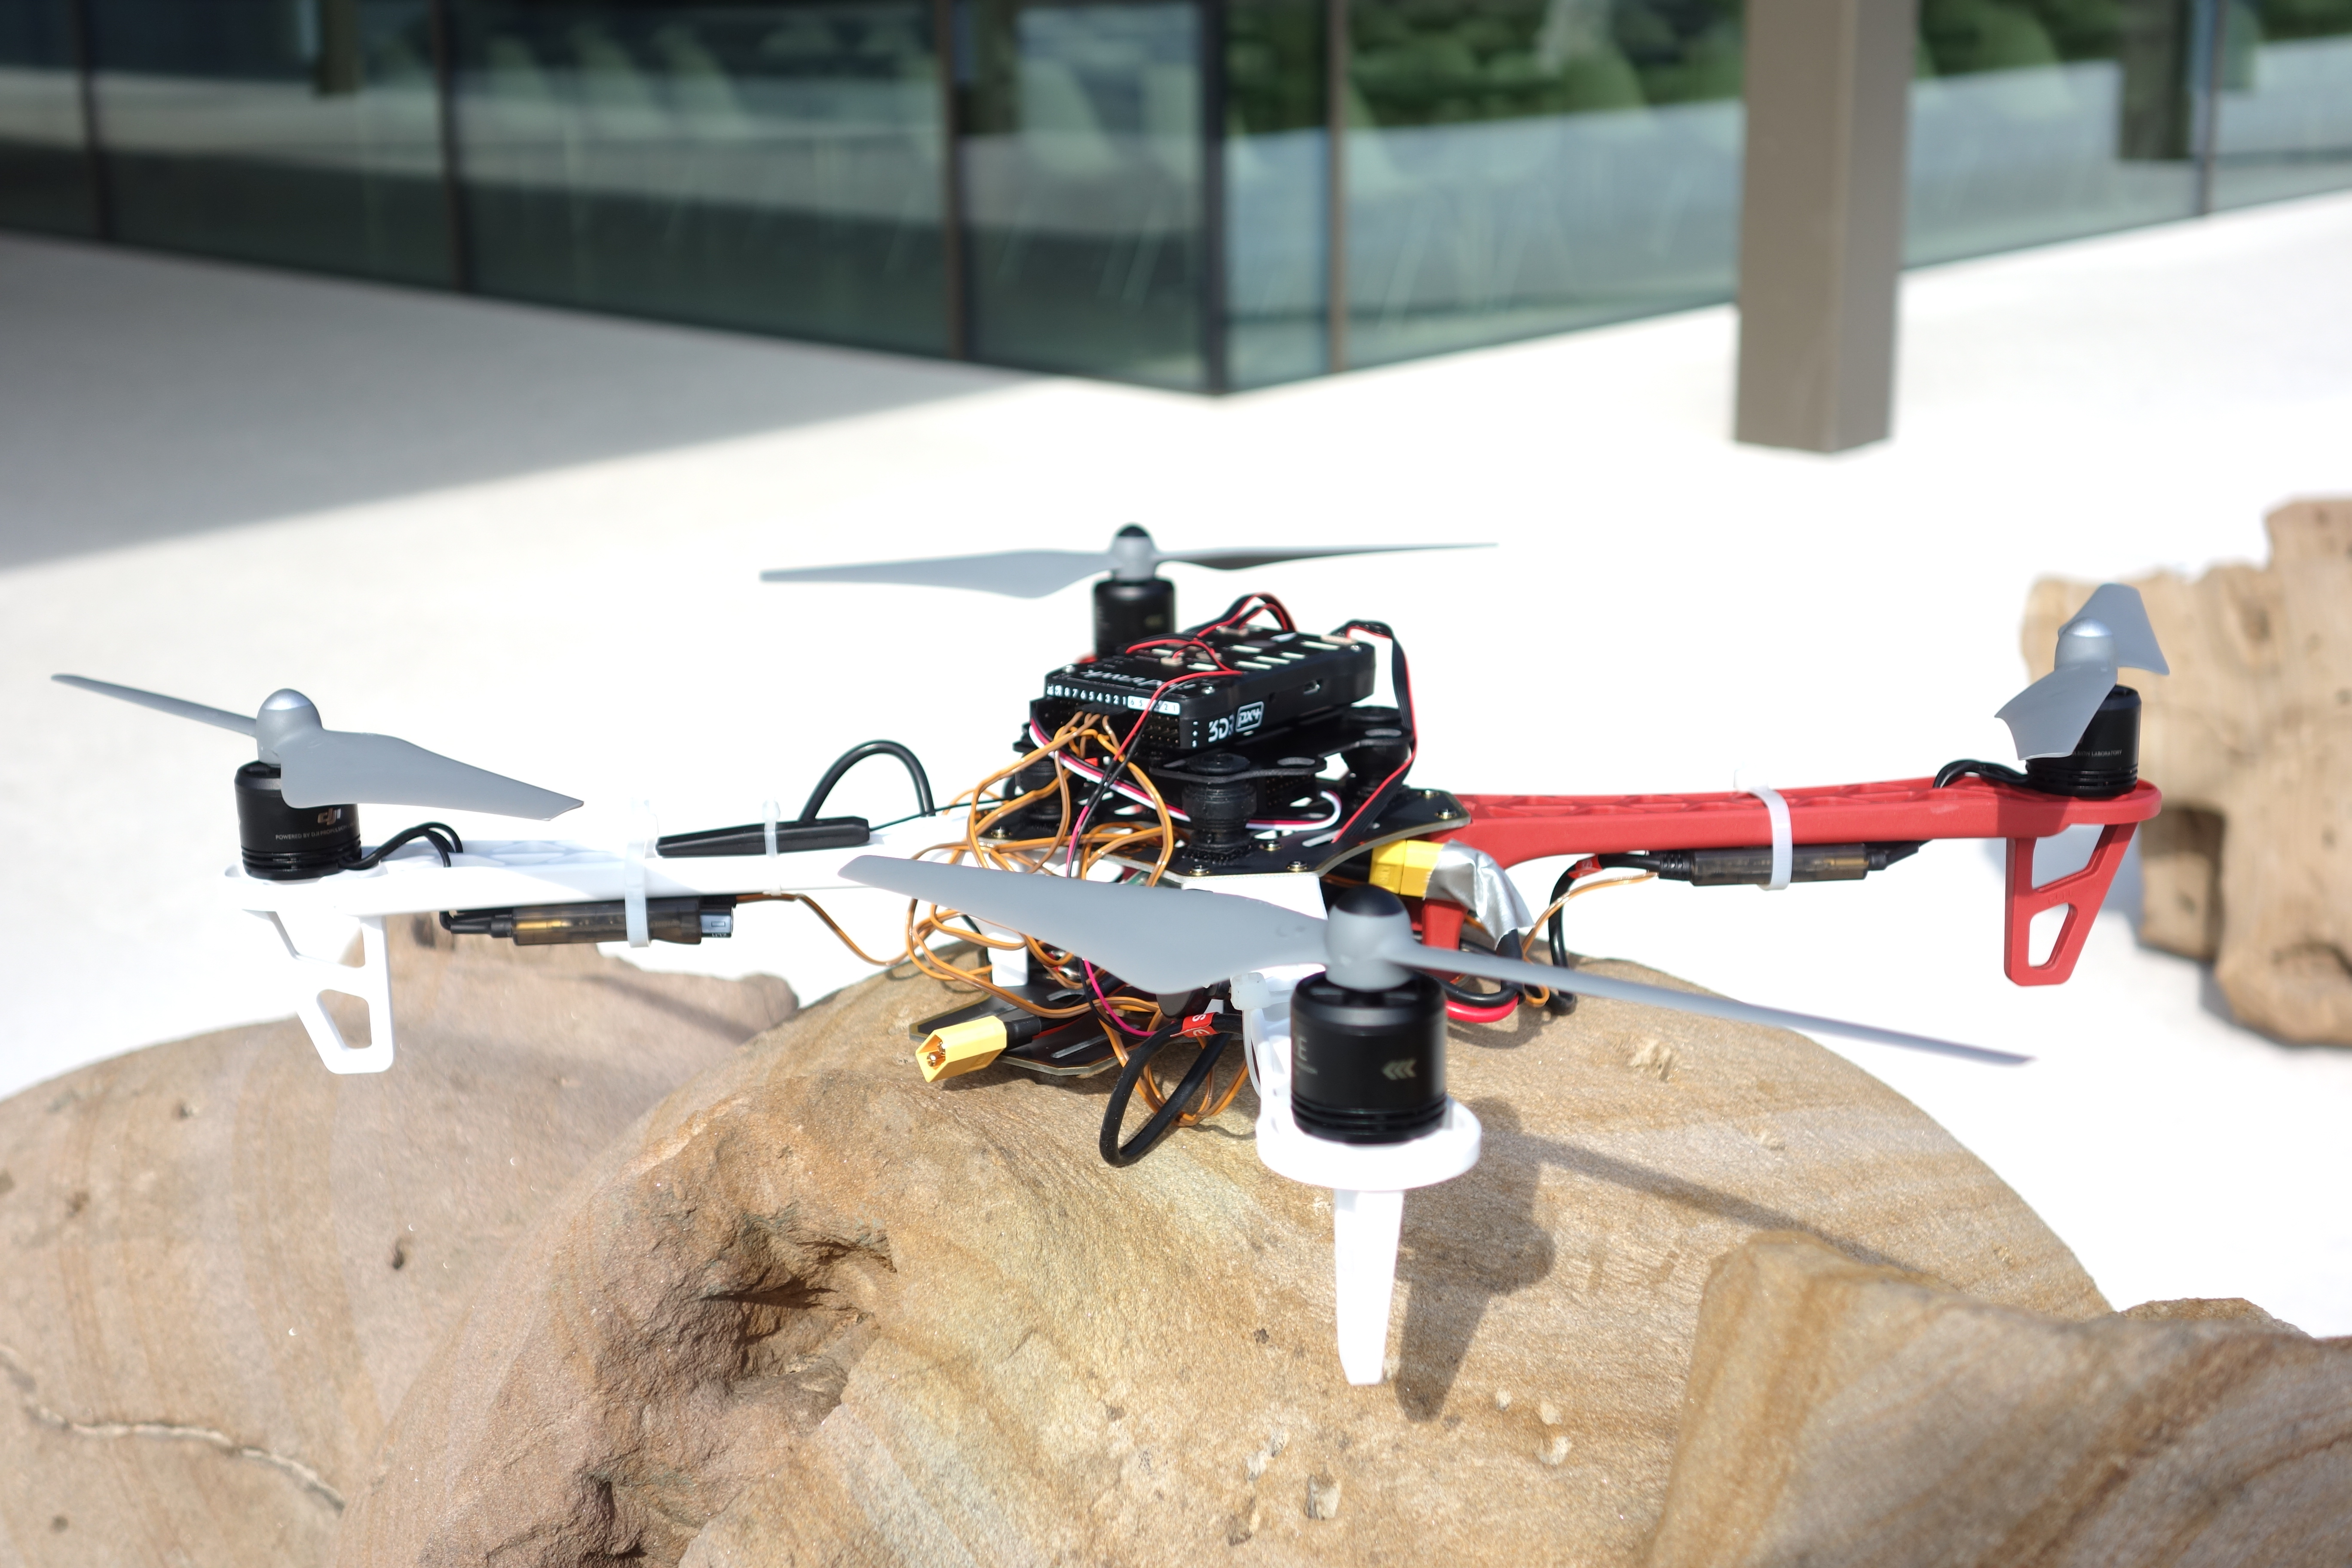
\includegraphics[width=0.9\textwidth] {images/hardware/prototype1.jpg} 
	\caption{Erster Prototyp ohne Landegestellt und ohne Smartphone}
	\label{fig:prototyp-1}
\end{figure}


\section{Libraries}

\subsection{Server}


\subsection{Onboard App}
\begin{tabularx}{\textwidth}{|X|X|c|c|}
	\hline
	\textbf{Name} & \textbf{Verwendungszweck} & \textbf{Version} & \textbf{Lizenz} \\
	\hline \hline
	DroneKit-Android Client library & Android API für MAV-Link Protokoll (Ansteuerung der Drohne) & 1.5.1 & Apache 2.0\\
	\hline 
\end{tabularx}
\subsection{User App}




\part{Anhang}
\newpage
\renewcommand \thechapter{\Alph{chapter}}


\chapter{Projektplan}
\section{Änderungsgeschichte}
\begin{tabularx}{\textwidth}{|c|c|X|c|}
  \hline
  \textbf{Datum} & \textbf{Version} & \textbf{Änderung} & \textbf{Autor} \\
  \hline \hline
  26.02.2016 & 1.0 & Erstellen des Projektplans & Martin Stypinski \\
  \hline
\end{tabularx}

\section{Einleitung}
\subsection{Ziel und Zweck}
Ziel dieser Arbeit ist \textit{Project-Helin} umzusetzten. 

\subsection{Lieferumfang}
Der Lieferumfang dieser Arbeit entspricht den Vorgaben der HSR:
\begin{itemize}
	\item{Zu Handen des Betreuers:
	\begin{itemize}
		\item{Ein gedrucktes Exemplar der Dokumentation}
		\item{Dokumentation, sämtliche Dokumente und Sourcen auf CD}
	\end{itemize}}
	\item{Poster - Enthält Zusammenfassung der Arbeit}
	\item{Abstract für die Bachelorarbeitsbrochure}
\end{itemize}
Zusätzlich ist es uns ein Anliegen, dass der Sourcecode und die Erfahrungen über den Zeitraum der Bachelorarbeit hinaus bestehen bleiben. Daher wurde ein github-repository eingerichtet, dass nach beendigung der Arbeit sämtliche Teile enthält: \textbf{\url{https://github.com/Project-Helin}}

\subsection{Annahmen und Einschränkungen}
Es kann angenommen werden, dass der Zeitplan im Rahmen der regulären Bachelorarbeit Zeit gültig ist. Es wird dabei berücksichtigt das ein Zeithorizont von 17 Wochen zuverfügung steht und die maximale Arbeitszeit von 360 Stunden pro Person nicht überschritten werden soll.

\section{Projektorganisation}
\subsection{Organisationsstruktur}
\begin{tabularx}{\textwidth}{|c|c|X|}
  \hline
  \textbf{Name} & \textbf{E-Mail} & \textbf{Verantwortung} \\
  \hline \hline
  Prof. Dr. Markus Stolz & \url{markus.stolze@hsr.ch} & Betreuer der Arbeit\\
  \hline \hline
  Marcel Amsler & \url{marcel.amsler@hsr.ch} & \\
  \hline
  Kirusanth Poopolasingam & \url{kirusanth.poopalasingam@hsr.ch} & \\
  \hline
  Martin Stypinski & \url{martin.stypinski@hsr.ch} & \\
    \hline
\end{tabularx}

\section{Risikomanagement}
\subsection{Risiken}
\LTXtable{\textwidth}{risk.tex}

\subsection{Umgang mit Risiken}
\begin{figure}[htbp]
\centering
\includegraphics{images/risk_result.png}
\caption{Risiko Matrix}
\label{Risk result}
\end{figure}


\subsection{Massnahmen}

\section{Meilensteinplanung}


\chapter{Sitzungsprotokolle}
%\includepdf[pages=-]{chapter/52protocol/protokoll_w01.pdf} 




\end{document}